\section{Platforms}
The suitable platforms for this project are examined in the following section. These platforms are capable of executing instructions as well as reading or writing to pins available on the board. These pins can be connect to components such as sensors and actuators.

\subsection{Arduino}\label{sec:arduino}
Arduino is an open source platform, which makes the software and hardware documentation available to the public. The name "Arduino" covers both the software platform and the range of hardware platforms with boards of different sizes, from the smaller Arduino Nano up to the Arduino Mega. One of the more popular Arduino boards is the Arduino Uno which is a medium sized board, often used by starters \cite{arduinouno}.

How the Arduino handles or reacts to input is implemented by the user and uploaded to the Arduino board by using the Arduino IDE.

\textbf{Arduino Uno}\\
One of the most common Arduino boards is the Uno, seen in figure \ref{fig:arduinouno}, which uses the ATmega328 microcontroller \cite{arduinouno}. It has 14 digital input/output pins, and 6 analog inputs for connecting different components. Considering specifications, which is shown in table \ref{tab:arduspecs}, the Uno is limited on its resources. Therefore it is needed to limit both program and data size, and also the amount of complex tasks.

\begin{figure}[h!]
\centering
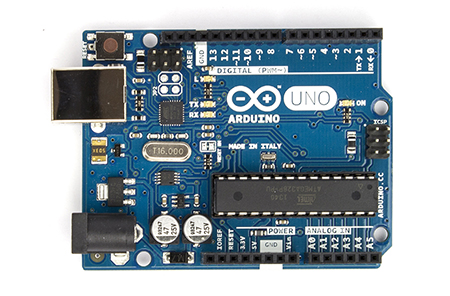
\includegraphics[width=0.5\textwidth]{chapters/analysis/figs/ArduinoUno.jpg}
\caption{The Arduino Uno board\cite{arduinointroduction}.}
\label{fig:arduinouno}
\end{figure}

\bgroup
\def\arraystretch{1.1}
\begin{table}[ht!]
%	\centering
	\begin{tabular}{p{15em} c c}
		Unit                        & Arduino Uno                                                                 & Arduino Mega                                                               \\ \hline
		Microcontroller             & ATmega328                                                                   & ATmega1280                                                                 \\
		Clock Speed                 & \multicolumn{2}{c}{16 MHz} \\
		Operating Voltage           & \multicolumn{2}{c}{5V}                                                                                                                                   \\
		Input Voltage (recommended) & \multicolumn{2}{c}{7-12V}                                                                                                                                \\
		Input Voltage (limits)      & \multicolumn{2}{c}{6-20V}                                                                                                                                \\
		DC Current per I/O Pin      & \multicolumn{2}{c}{40 mA}                                                                                                                                \\
		DC Current for 3.3V Pin     & \multicolumn{2}{c}{50 mA}                                                                                                                                \\
		Analog Input Pins           & 6                                                                           & 16                                                                         \\
		Digital I/O Pins            & \begin{tabular}[t]{@{}c@{}}14\\ (6 provide PWM output)\end{tabular}         & \begin{tabular}[t]{@{}c@{}}54\\ (15 provide PWM output)\end{tabular}       \\
		Flash Memory                & \begin{tabular}[t]{@{}c@{}}32 KB\\ (0.5 KB used by bootloader)\end{tabular} & \begin{tabular}[t]{@{}c@{}}128 KB\\ (4 KB used by bootloader)\end{tabular} \\
		SRAM                        & 2 KB                                                                        & 8 KB                                                                       \\
		EEPROM                      & 1 KB                                                                        & 4 KB                                                                       \\                
	\end{tabular}
	\caption{Arduino Uno and Mega specifications \cite{arduinouno}\cite{arduinomega}.}
\end{table}\label{tab:arduspecs}
\egroup

\iffalse%udkommenteret
\begin{table}
\begin{tabular}{| l | l |}
\hline
Microcontroller & ATmega328\\
Operating Voltage & 5V\\
Input Voltage (recommended) & 7-12V\\
Input Voltage (limits) & 6-20V\\
Digital I/O Pins & 14 (of which 6 provide PWM output)\\
Analog Input Pins & 6\\
DC Current per I/O Pin & 40 mA\\
DC Current for 3.3V Pin & 50 mA\\
Flash Memory & 32 KB (ATmega328) of which 0.5 KB is used by bootloader\\
SRAM & 2 KB (ATmega328)\\
EEPROM & 1 KB (ATmega328)\\
Clock Speed & 16 MHz\\
\hline
\end{tabular}
\caption{Specifications for the Arduino Uno\cite{arduinouno}.}
\end{table}
\label{tab:unospec}
\fi

\textbf{Arduino Mega}\\
The Arduino Mega is a larger version of the Uno. The Mega has more memory and pins, which makes it better for handling larger programs and amounts of data, and also allows more components to be connected to the board. Since the clock speed is the same as the Uno, the Mega will not process data faster\cite{ardcomp}.

\begin{figure}[h!]
\centering
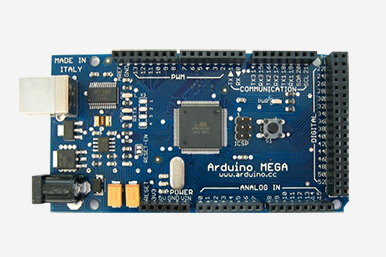
\includegraphics[width=0.6\textwidth]{chapters/analysis/figs/ArduinoMega.jpg}
\caption{The Arduino Mega board\cite{arduinomegaimg}.}
\label{fig:arduinomega}
\end{figure}

\iffalse%udkommenteret
\begin{table}[h!]
\begin{tabular}{| l | l |}
\hline
Microcontroller & ATmega1280\\
Operating Voltage & 5V\\
Input Voltage (recommended) & 7-12V\\
Input Voltage (limits) & 6-20V\\
Digital I/O Pins & 54 (of which 15 provide PWM output)\\
Analog Input Pins & 16\\
DC Current per I/O Pin & 40 mA\\
DC Current for 3.3V Pin & 50 mA\\
Flash Memory & 128 KB of which 4 KB used by bootloader\\
SRAM & 8 KB\\
EEPROM & 4 KB\\
Clock Speed & 16 MHz\\
\hline
\end{tabular}
\caption{Specifications for the Arduino Mega\cite{arduinomega}.}
\end{table}
\label{tab:megaspec}
\fi


\subsection{Raspberry Pi}
Raspberry Pi is a series of single board computers. The Raspberry Pi series contains some powerful controllers compared to other pocket sized processing units.

The Raspberry Pi has a set of pins for connecting to external hardware. There are four different pin types available; two 5v power, two 3.3v power, five ground and 17 GPIO. In \figref{abPins} the placement of the pins is shown. 

The GPIO, or "general purpose input/output" pins can be used to either send or receive digital signals. Unlike the Arduinos it is stricly digital, as it does not have a build in analog to digital converter. If analog input processing is needed, this will have to be done externally.

\begin{figure}[H]
\centering
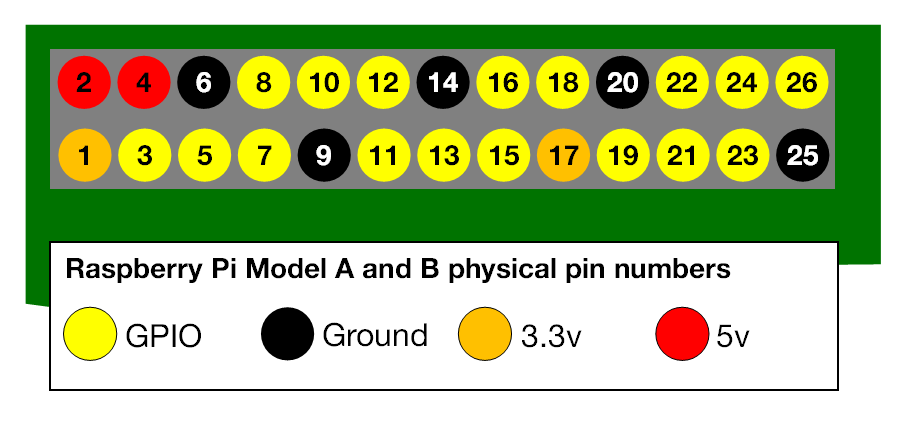
\includegraphics[width=0.6\textwidth]{chapters/analysis/figs/rpiABPins.png}
\caption{Raspberry Pi pins on model A and B.}
\label{fig:abPins}
\end{figure}

Because of the computing power and memory of a Raspberry Pi, a Linux OS is usually installed on the Raspberry Pi\cite{Arduino_linux}. A Raspberry Pi also has a GPU, video output, and USB port.

\textbf{Raspberry Pi B+}\\
In this subsection a Raspberry Pi B+ will be described as these were available to use in the project. The different models usually differs on CPU speed and memory.

The Raspberry Pi B+ specifications are shown in table \ref{tab:pibplusspec}. Futhermore the B+ also contains HDMI video output and Ethernet connectivity. A micro SD card is used as main storage a micro, which contains the OS.

\begin{figure}[H]
\centering
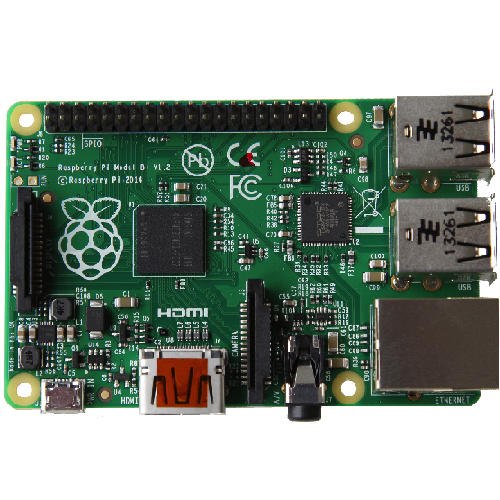
\includegraphics[width=0.6\textwidth]{chapters/analysis/figs/raspberry-pi-model-b-plus.png}
\caption{Raspberry Pi B+\cite{pibplus}.}
\label{fig:pibplus}
\end{figure}

\begin{table}[H]
\centering
\begin{tabular}{| l | l |}
\hline
Microcontroller & Broadcom BCM2835\\
RAM & 512MB\\
Extended GPIO Pins & 40\\
USB Ports & 4\\
Clock Speed & 700 MHz\\
\hline
\end{tabular}
\caption{Specifications for Raspberry Pi B+\cite{pispecs}.}
\end{table}
\label{tab:pibplusspec}
